\chapter{Segmentation\\ (Timothé)}

Pour la première soutenance, nous avons décidé de commencer par traiter le cas
de textes pré-formatés, à savoir un texte droit où les caractères ne se
touchent pas et où chaque ligne est délimitée par un vide.

\section{Détection de lignes}

L'algorithme initial avec cette supposition est donc relativement simple et son
implémentation modulaire. La fonction prend une image en entrée, et découpe
horizontalement la prochaine ligne tant qu'aucune ligne entièrement blanche
n'est détectée. Cette partie rectangulaire de l'image est ensuite extraite, puis
passée en paramètre de la fonction de découpe des caractères.

\begin{figure}[H]
    \centering
    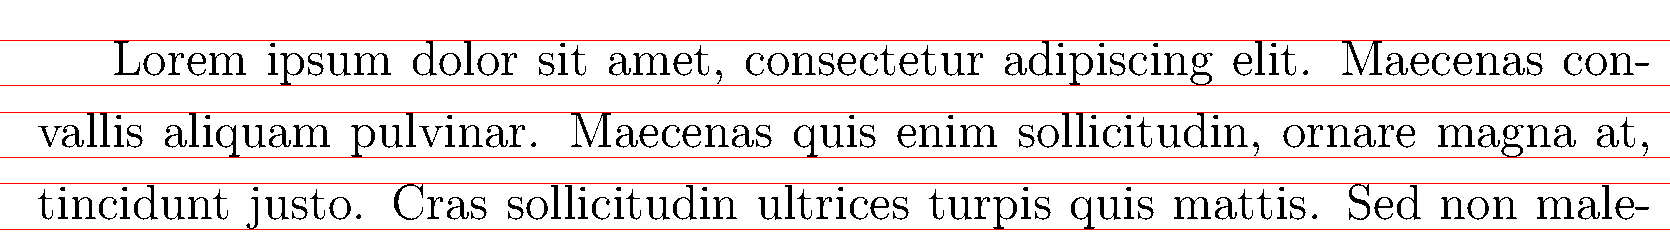
\includegraphics[width=1\textwidth]{segmentation_line}
    \caption{Segmentation des lignes}
\end{figure}

\section{Détection de caractères}

D'une manière similaire, en utilisant comme entrée une ligne de texte, la
fonction effectue une découpe verticale pour segmenter la ligne en différents
caractères. Ces derniers seront par la suite envoyés au réseau de neurones (une
fois entraîné).

\begin{figure}[H]
    \centering
    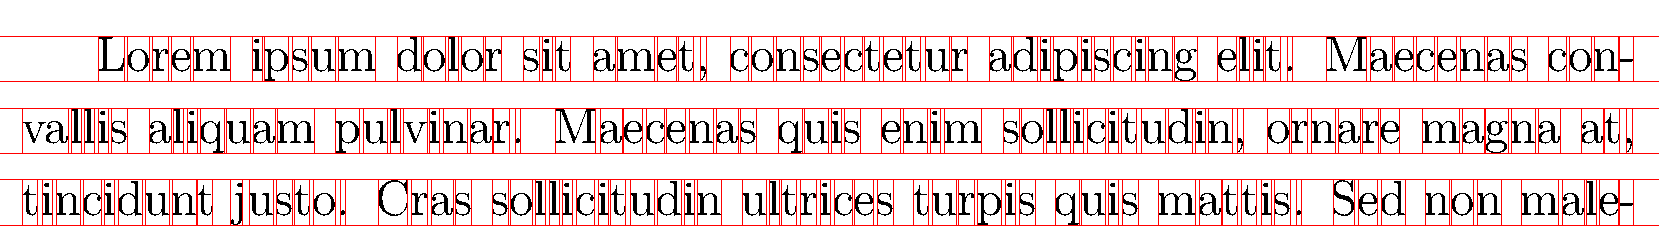
\includegraphics[width=1\textwidth]{segmentation_char}
    \caption{Segmentation des caractères}
\end{figure}

Une première implémentation de ces fonctions utilisait la représentation
matricielle, mais il a été décidé de garder cette dernière une fois toutes les
opérations sur les images traitées pour uniquement faire la correspondance avant
le réseau de neurones. Cela facilite davantage la gestion des images, des
différents formats, et des tests des fonctions notamment.
